\chapter{Methodology}
\label{ch:methodology}

The approach that this project will undertake is a mixture of a iterative design and prototyping process, which is then evaluated to seek the answer of the given research question.

\section{Design process}
\label{sec:designprocess}

The design process will focus on iterating over designs and prototypes in a user-centered manner. By conducting an iterative design process, the design will be improved upon repetitively -- starting from low-fidelity sketches and ending at high-fidelity prototypes.

Using this method, stakeholders and potential users will be able to try out the design throughout various phases of its development. This user testing may consist of focus groups and uncontrolled experiments, and the gained experience can be applied in the next development stage. In this case, the testing will be restricted to an internal group at first, involving other users once the project hits its evaluation stage.

In addition, heuristics are used to analyse elements that are not thoroughly investigated during the design process. Heuristic evaluation is about evaluating a user interface based on a set of heuristics, that is, usability principles or simply rules of thumb. Some examples include \enquote{error prevention} and \enquote{recognition rather than recall} \parencite{nilsen1994}. Such evaluation can be performed by a single person, as long as said person follows a predefined set of heuristics.

This process may function as a initial part of the application development. Ideas are sought for and discovered, then shaped into designs that form a basis for a software development phase. Looking into the \enquote{double diamond} design process model \parencite{designcouncil2007}, this can be viewed as the first two stages shaping the first diamond. This model is built on the idea of going from a generic problem statement to defining specific problems and then creating specific solutions for said problems, diverging and converging the area of focus during the process.

\begin{figure}
    \centering
    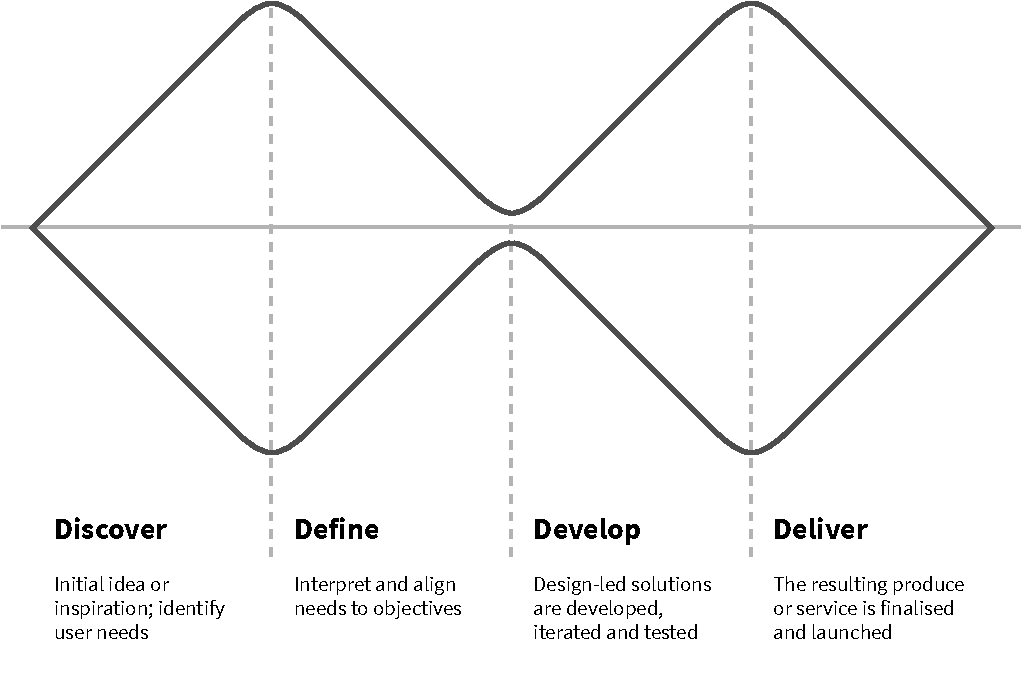
\includegraphics[width=0.8\textwidth]{double-diamond.pdf}
    \caption{The \enquote{double diamond} design process model}
    \label{fig:doublediamond}
\end{figure}

% For hver iterasjon
% - Hva er problemstillingen?
% - Hvilken tilnærming til løsningen skal prototypen ha?
% - Hvordan er det levert?
% - Hvordan det er testet/testresultater

% Må utforske mye før man fokuserer inn på problemstilling - utforskningen er iterativ

\section{Interaction design}
\label{sec:interactiondesign}

The idea of iterating a design while putting the user in the front seat is also key in interaction design. As the name suggests, this method is about emphasizing and facilitating interaction between humans and computers. Close monitoring by user testing is important to see if interactions with an application succeed. \textcite{preece2015} developed a lifecycle model for interaction design that can illustrate the iterative process used in this project. This model is shown in \autoref{fig:interactiondesign}. (...)

% Forklar mer

\begin{figure}
    \centering
    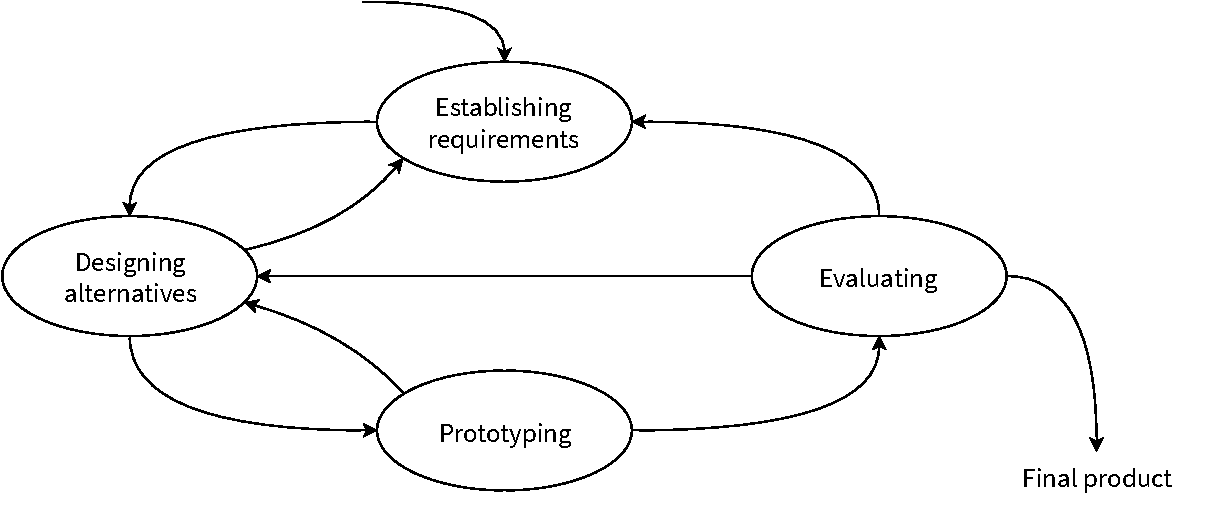
\includegraphics[width=0.8\textwidth]{interaction-design-lifecycle-model.pdf}
    \caption{Interaction design lifecycle model}
    \label{fig:interactiondesign}
\end{figure}

\section{Prototyping}
\label{sec:prototyping}

A prototype in this sense is an early version of the product or the application. It does not mean that the prototype needs to be interactive, although a prototype certainly may be. During an iterative design process, each iteration leads to a new and improved prototype that may be tested. Basic prototypes with plain visuals are called \emph{low fidelity} while more polished prototypes are \emph{high fidelity}. Following are a few types of prototypes mentioned in this document:

\begin{description}
    \item[Form study prototype] is a prototype with more focus on geometry and less focus on colours and detail. Prototypes are normally considered low-fidelity at this stage.
    \item[Functional prototype] has an emphasis on the functional aspects of the application, but also the visual appearance of it. Such prototypes should be close to indistinguishable from a final product, although it may be made in a different shape or form.
    \item[Interactive prototype] means that the prototype may be interacted with through use of equipment (keyboard, mouse \emph{et cetera}), tactile movements (touch, gestures \emph{et cetera}) or by other means. The interaction should help the user accomplish their goals of using the application.
\end{description}

\subsection{Prototyping tools}

Prototypes may be made with a wide selection of tools. The most basic ones may be created by simply using pen and paper. This may be sufficient to create something interactive, using several sheets of paper to change the prototype's appearance.

Dedicated prototyping software come in handy for more high-fidelity prototypes. Most prototyping applications are based on a set of screens with hotspots linking them together. A hotspot defines an area to click or tap on, leading the user to the desired screen -- optionally coupled with an animation. % Prototyping software that have been used in this project are \emph{Marvel} for earlier iterations and \emph{Figma} for later ones.

% Marvel
% Figma

\section{Evaluation}
\label{sec:evaluation}

This project functions as a pilot study in preparation for a bigger project held at the Children and Youth Clinic. It is also an explorative study as it may discover new ways to communicate between patients and the hospital, possibly supplementing the current way of informing patients. This will allow the clinic to run a small-scale project and see how the application compares to the existing systems at an early stage with reduced investment and costs.

The final prototype will be evaluated by a usability test. A small group will be invited to test and evaluate the application. The users are to be handed an interactive prototype and asked to use it at their will. In addition, the users will give their impressions of the system through a semi-structured interview. These questions, if not already answered, are centered around topics such as \emph{informing}, \emph{ease of use} and \emph{trust}. The results are to be analysed qualitatively.

% The project is deemed to be valuable if the users find the application to be more informative and engaging than the current system.
